\documentclass{beamer}

\usepackage{default}
\usepackage[german]{babel}
\usepackage[utf8]{inputenc}                   % replace by the encoding you are using

\usetheme{Berlin}

%Header Settings
%\setbeamertemplate{headline}{}

%Footer Settings
\setbeamertemplate{navigation symbols}{
	\usebeamerfont{footline}%
	\usebeamercolor[fg]{footline}%
	\hspace{1em}%
	\insertframenumber/\inserttotalframenumber
}

\title[Java]{Java - Variables}
\author[W. Bombardelli]{William Bombardelli}
\institute[Schweizerschule Mexiko]
{
	\vskip 12pt
	Schweizerschule Mexiko, Ciudad de México, Mexico \\
	\texttt{\url{https://github.com/wbombardellis/java-unterricht}}
}
\date{25 September 2019}

\makeatletter
\hypersetup{
	pdftitle = {\@title}, pdfkeywords = {Java}, pdfauthor = {\@author}
} 
\makeatother

\begin{document}
	\begin{frame}
		\titlepage
	\end{frame}
	
	\begin{frame}
		\frametitle{Organization}
		\tableofcontents
	\end{frame}

	%-------------------
	% Review
	%-------------------
	\begin{frame}
		\frametitle{Algorithm Review}
		\url{https://www.youtube.com/watch?v=CvSOaYi89B4} (Until 3:12)
	\end{frame}
	
	%-------------------
	% Model of Computation
	%-------------------
	\section{Model of Computation}
	\begin{frame}
		\frametitle{Model of Computation}
		\centering
		\vspace{-4px}
		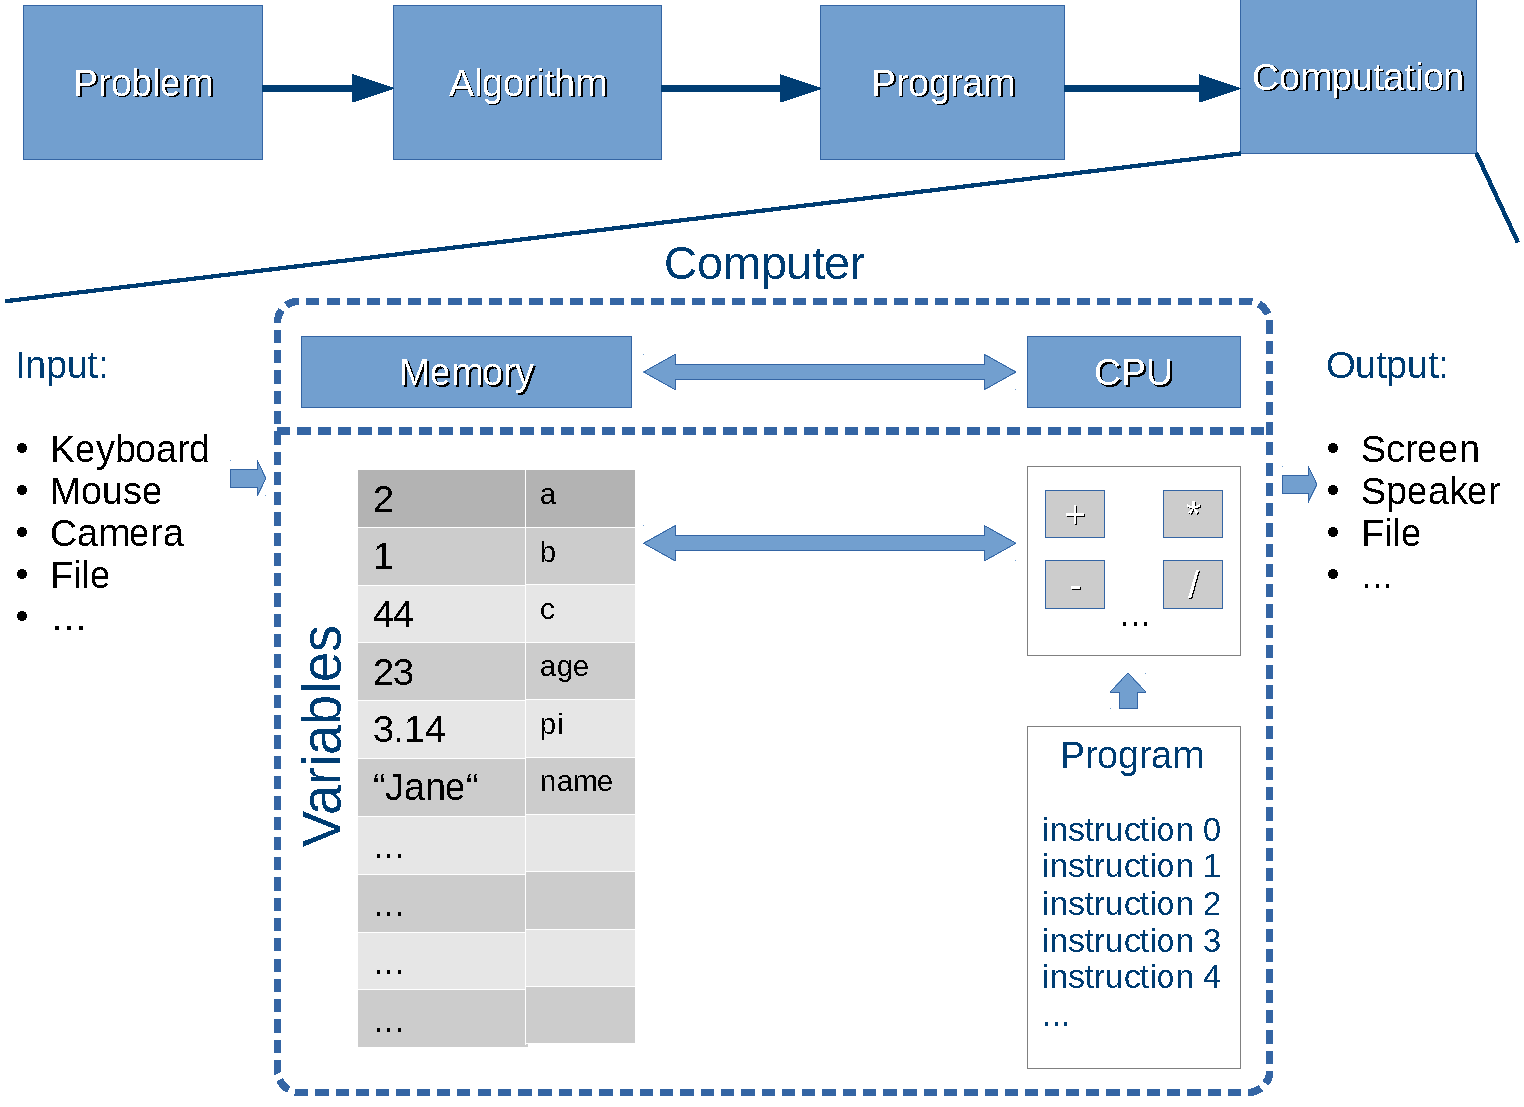
\includegraphics[width=.9\textwidth]{Memory-CPU-Scheme}
	\end{frame}

	%-------------------
	% Variables
	%-------------------
	\section{Variables in Java}

	\begin{frame}
		\frametitle{Variables in Java}
		$int\ a;$\\
		$a = 10;$\\
		$int\ b;$\\
		$b = 1;$\\
		$int\ c;$\\
		$c = a + b;$\\
		$System.out.println(c);$
	\end{frame}

	\begin{frame}
		\frametitle{Variables in Java with Input}
		$Scanner\ reader = new\ Scanner(System.in);$\\
		$int\ a =reader.nextInt();$\\
		$int\ b = 1;$\\
		$int\ c = a + b;$\\
		$System.out.println(c);$
	\end{frame}

	\begin{frame}
		\frametitle{Exercises}
		\begin{itemize}
			\item Write a program in Java that reads two integer values from the keyboard and prints their sum, difference, product and division at the screen/ console.
			\pause
			\item Write a program in Java that calculates and prints the area $A$ of a triangle after reading its base $b$ and height $h$ from the user's keyboard. Remember: $A = \frac{b \times h}{2}$
			\pause
			\item Write a program in Java that calculates and prints the area $A$ of a triangle with side lengths $a, b$ and $c$. For that you can use the Heron's formula $A = \sqrt{s \cdot (s-a) \cdot (s-b) \cdot (s-c)}$ where $s = \frac{a+b+c}{2}$ is the semi-perimeter of the triangle.
		\end{itemize}
	\end{frame}

	
	%-------------------
	% Summary
	%-------------------
	\section{Summary}

	\begin{frame}
		\frametitle{Summary}
		\centering
		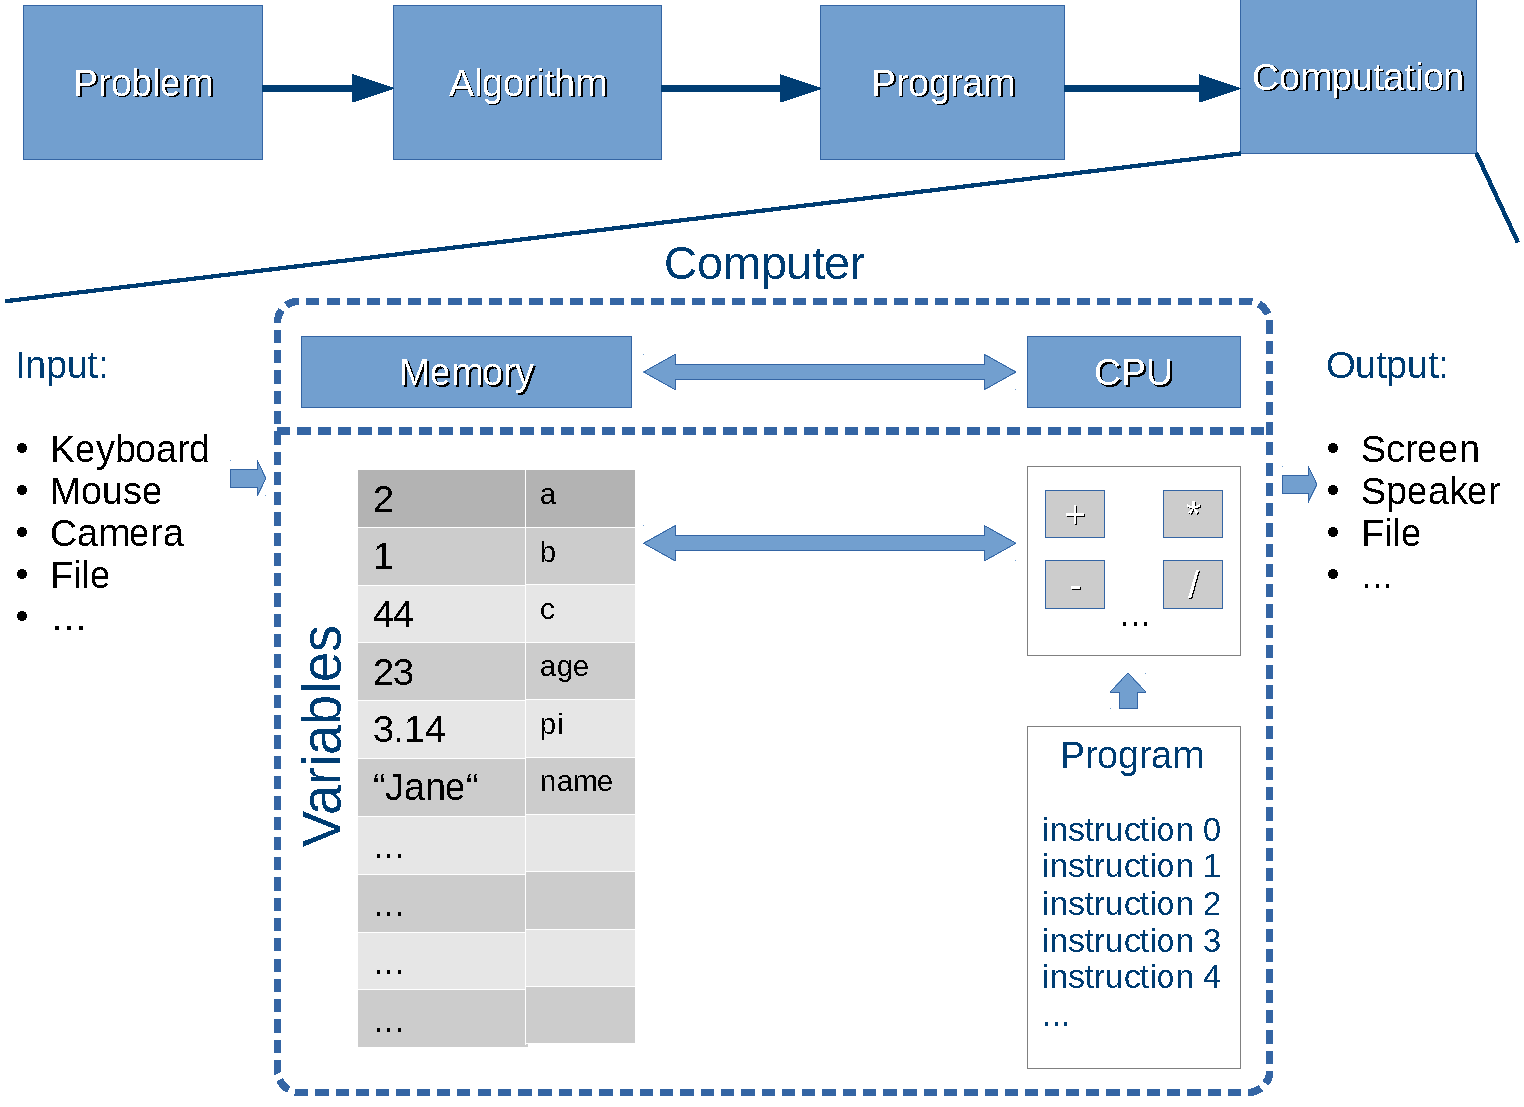
\includegraphics[width=.7\textwidth]{Memory-CPU-Scheme}
		\begin{itemize}
			\item Next Week: Data Types
		\end{itemize}
	\end{frame}

	\begin{frame}
		\frametitle{References}
		\begin{itemize}
			\item W3C Tutorial: 
			\begin{itemize}
				\item \url{https://www.w3schools.com/java/java\_variables.asp}
				\item \url{https://www.w3schools.com/java/java\_operators.asp}
				\item \url{https://www.w3schools.com/java/java\_math.asp}
			\end{itemize}
			\item Exercises: \url{https://www.w3schools.com/java/exercise.asp}
			\begin{itemize}
				\item Java Variables
				\item Java Operators
			\end{itemize}
		\end{itemize}
	\end{frame}

\end{document}
